\documentclass[letterpaper, 12pt] {article}

\usepackage{amsmath}
\usepackage{graphicx}
\usepackage{wrapfig}
\usepackage[margin=2cm]{geometry}
\usepackage[export]{adjustbox}
\usepackage{caption}
\usepackage{subcaption}
\usepackage[spanish, es-tabla]{babel}
\usepackage[T1]{fontenc}
\usepackage[utf8]{inputenc}
\usepackage{physics}
\usepackage[shortlabels]{enumitem}
\usepackage{multicol}

\usepackage{xcolor} 
	\definecolor{bone}{RGB}{253,255,224}  %hueso
	\definecolor{lgreen}{RGB}{146,197,130} %light green,
	\definecolor{lblue}{RGB}{134,165,169} %light blue
	\definecolor{lgray}{RGB}{118,118,118} %light gray
	\definecolor{dgreen}{RGB}{83,111,80}%dark green
	
\usepackage[colorlinks, linkcolor=lblue]{hyperref}
\graphicspath {{images/}}	
	
\usepackage[most]{tcolorbox}
\tcbset{%colback=blue!55!green, colframe= blue!55!green,
		colback=lgreen, colframe= dgreen,
		  colbacktitle = green!50!blue, sharp corners = downhill, 
	  fonttitle=\bfseries , boxrule = .75mm }%,leftrule = 5mm}

\newcommand{\er}{\ensuremath{\hat{e}_r}}


\title{\LARGE \bf 
Coeficientes de esparcimiento: Esfera en presencia de una onda plana con $\lambda\gg 1$}
\author{Urrutia Aguiano, Jonathan Alexis}
\date{}
\begin{document}
\maketitle

La solución de Mie trata el problema de una onda plana que incide en una partícula esférica de tamaño arbitrario. En particular, el límite de partícula pequeña, que es equivalente al de longitud de onda grande, reproduce resultados conocidos de la electrostática: el de una esfera en un campo eléctrico constante. En este texto se corrobora esta afirmación.

\section{Caso estático: Esfera en un campo constante}

Supóngase una esfera esfera dieléctrica con una función dieléctrica $\varepsilon_D$ y radio $a$, inmersa en un  medio caracterizado por su función dieléctrica $\varepsilon_f$, que es sometida a un campo eléctrico constante 
\begin{equation}
\vec{E}^{i} = E_0 \hat{e}_z,
\end{equation}
como se muestra en la fig. \ref{fig:est}. Para calcular el campo eléctrico en todo el espacio, se resuelve la ecuación de Laplace considerando simetría azimutal, es decir, el potencial eléctrico está dado como
\begin{equation}
\phi (\vec{r}) = \sum_{l=0}^\infty  \left(A_l r^l + \frac{B_l}{r^{l+a}}\right)P_l(\cos\theta),
\end{equation}
donde $P_l(\cos\theta)$ son los polinomios de Legendre de grado $l$, una base ortogonal. 
\begin{figure}[h]\centering
\begin{minipage}{.8\linewidth}\centering
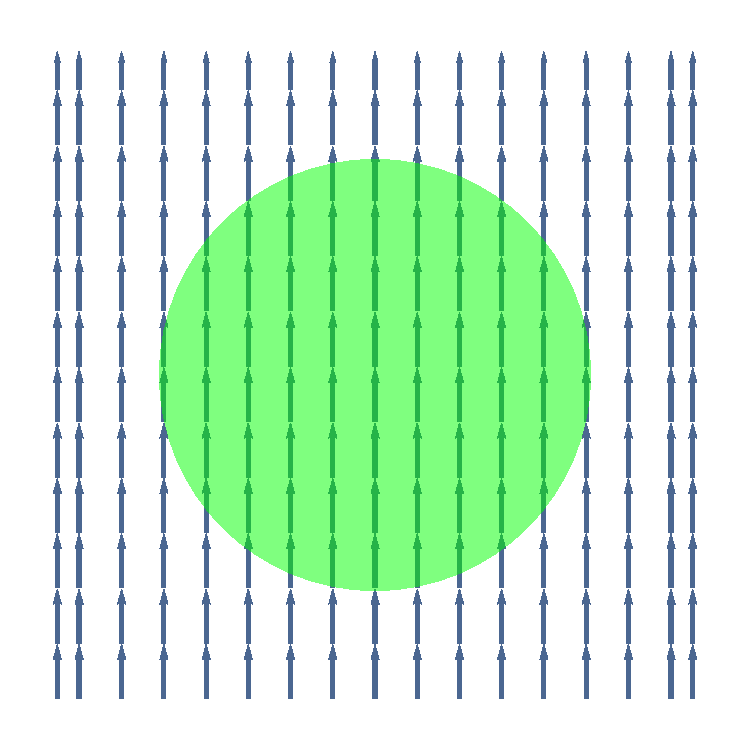
\includegraphics[width=4.5cm]{problemaEst}
\caption{\footnotesize  Esfera dieléctrica en presencia de un campo eléctrico constante.}
\label{fig:est}
\end{minipage}
\end{figure}


El potencial en todo el espacio puede dividirse en un potencial dentro de la esfera y uno fuera, es decir
\begin{equation}
\phi (\vec{r}) = \left\{ 
	\begin{array}{ll}
	\sum\limits_{l=0}^\infty A_l r^l P_l(\cos\theta)& \mbox{si } r<a,\\
	\sum\limits_{l=0}^\infty  \left( B_l r^l + \frac{C_l}{r^{l+a}}\right)P_l(\cos\theta) &\mbox{si }  a<r,
	\end{array} \right.\label{eq:phi}
\end{equation}
con las condiciones a la frontera

{\centering
\begin{enumerate}[(i)]
\item $-\frac{1}{a}\eval{\dv{ \phi_D}{\theta}}_a = -\frac{1}{a}\eval{\dv{ \phi_f}{\theta} }_a$,\label{item:Par}
\item $-\varepsilon_D \eval{\dv{ \phi_D}{r}}_a =-\varepsilon_f \eval{\dv{ \phi_f}{r}}_a$, \label{item:Perp}
\item Si $r\gg a$, entonces $\phi_f \to - E_0 z = - E_0 r\cos\theta$, \label{item:inf}
\end{enumerate}
}
donde la condición \ref{item:Par} es la continuidad de las componentes paralelas del campo eléctrico, la condición \ref{item:Perp} es la continuidad de las componentes normales del vector de desplazamiento y la condición \ref{item:inf} es el comportamiento asintótico.
 
Por la condición \ref{item:inf}, y dado que $P_1(\cos\theta)= \cos\theta$, se concluye que
	\begin{equation}
	B_1 = -E_0,\label{eq:B1}
	\end{equation} 
mientras que los coeficientes  $B_l$ para $l \not=1$ son nulos. Empleando las condiciones \ref{item:Par} y \ref{item:Perp} en la ec. \eqref{eq:phi}, se obtiene para $l = 1$
	\begin{subequations}
	\begin{align}
	A_1a &= B_1 a + \frac{C_1}{a^2}, \\
	\varepsilon_D A_1 & = \varepsilon_f \left( B_1 -\frac{2C_1}{a^3} \right),
	\end{align} \label{eq:A1}
	\end{subequations}	
y para $l \not= 1$
	\begin{subequations}
	\begin{align}
	A_la^l &= \frac{C_l}{a^{l+1}}, \\
	\varepsilon_D A_l a^{l-1} & = -\varepsilon_f \frac{C_l (l+1)}{a^{l+2}}. 
	\end{align} \label{eq:Al}
	\end{subequations}	
Para los coeficientes con $l \not= 1$, las ecs. \eqref{eq:Al} se satisfacen si $A_l = C_l = 0$. Sustituyendo la ec. \eqref{eq:B1} en las ecs. \eqref{eq:A1}, se calculan a las expresiones de los coeficientes $A_1$ y $C_1$, que son 
\begin{subequations}
\begin{align}
A_1 &= - \left( \frac{3}{2+m^2} \right) E_0,\\
C_1 &= \left(\frac{m^2-1}{m^2+2}  \right) E_0 a^3,
\end{align}\label{eq:A1C1}
\end{subequations}
con $m^2 = \varepsilon_D / \varepsilon_f = N_D^2/N_f^2$, donde $N_D$ es el índice de refracción dentro de la esfera y $N_f$ el índice de refracción afuera de la esfera; esto significa que se asume que la permeabilidad magnética de ambos medios es la misma.

Sustituyendo los coeficientes obtenidos [ec. \eqref{eq:A1C1}] en la ec. \eqref{eq:phi}, se obtiene una expresión del potencial eléctrico
\begin{equation}
\phi (\vec{r}) = \left\{ 
	\begin{array}{ll}
	- \left( \frac{3}{2+m^2} \right) E_0r\cos\theta& \mbox{si } r<a,\\
	-  E_0r\cos\theta + \left(\frac{m^2-1}{m^2+2}\right) E_0 a^3 \frac{\cos\theta}{r^2} &\mbox{si }  a<r.
	\end{array} \right.\label{eq:phiR}
\end{equation}
Nótese que el segundo término de la ec. \eqref{eq:phiR} cuando $a<r$ puede escribirse como un potencial dipolar ${\phi}_{dip}$, dado por
\begin{equation}
\phi_{dip} = \frac{1}{4\pi\varepsilon_f } \frac{\vec{p}\cdot\hat{e}_r}{r^2},
\end{equation}
si el momento dipolar fuese
\begin{equation}
\vec{p} = 4\pi\varepsilon_f \left(\frac{m^2-1}{m^2+2}\right)E_0 a^3 \hat{e}_z.
\end{equation}

Dado que el potencial escalar electrostático se relaciona con el campo eléctrico mediante la relación $\vec{E}=-\nabla\phi$,  el campo eléctrico producido por un dipolo (ver fig. \ref{fig:dip}) es
\begin{equation*}
- \nabla\phi_{dip} = \frac{p}{4\pi\varepsilon_f r^3} (2\cos\theta\hat{e}_r + \sin\theta\hat{e}_\theta).
\end{equation*}
\begin{figure}[t]\centering
\begin{minipage}{.8\linewidth}\centering
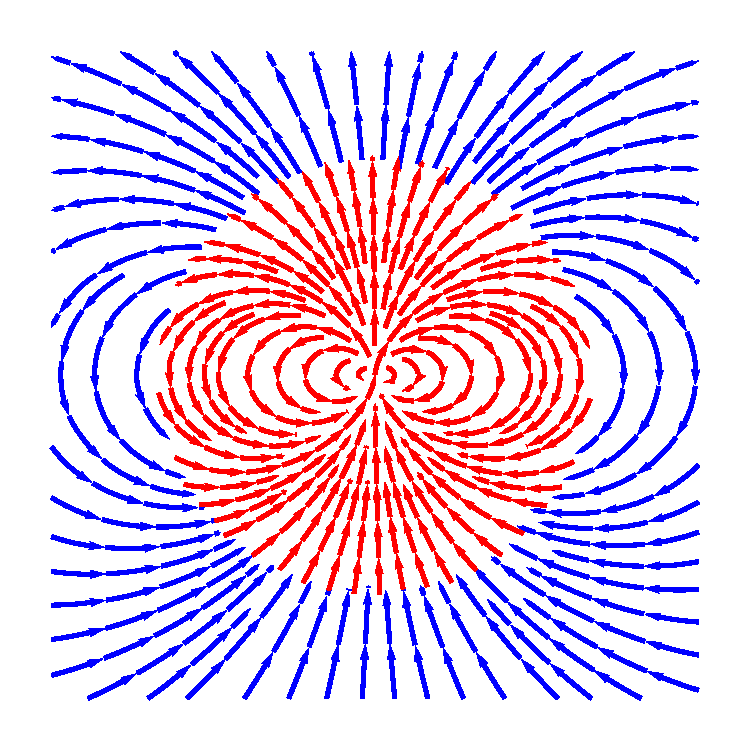
\includegraphics[width=4.5cm]{dipolo}
\caption{\footnotesize  Campo eléctrico producido por un dipolo. En rojo se se muestra el campo si $r<	a$ y en azul si $r>a$.}
\label{fig:dip}
\end{minipage}
\end{figure}
Calculando entonces el campo eléctrico a partir del potencial eléctrico [ec. \eqref{eq:phiR}], se obtiene que el campo eléctrico en todo el espacio está dado por
\begin{equation}
\vec{E} (\vec{r}) = \left\{ 
	\begin{array}{ll}
	\left( \frac{3}{2+m^2} \right) E_0 \hat{e}_z & \mbox{si } r<a,\\
	 E_0\hat{e}_z + \left(\frac{m^2-1}{m^2+2}\right)\frac{E_0 a^3}{r^3} (2\cos\theta\hat{e}_r + \sin\theta\hat{e}_\theta) &\mbox{si }  a<r,
	\end{array} \right.\label{eq:Eest}
\end{equation}
como se muestra en la fig. \ref{fig:Eest}. Nótese que el campo cuando $r<a$ es un campo constante y que el campo fuera de la esfera tiene una contribución del campo externa más una contribución dipolar.
\begin{figure}[h]\centering
\begin{minipage}{.8\linewidth}\centering
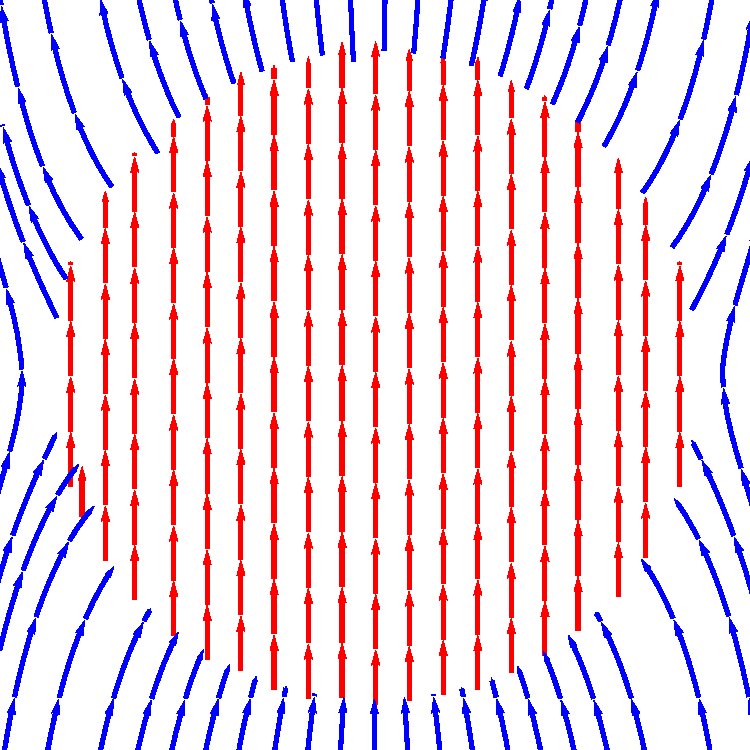
\includegraphics[width=4.5cm]{campoEst}
\caption{\footnotesize  Campo eléctrico total de una esfera en presencia de un campo externo uniforme.  En rojo se se muestra el campo si $r<	a$ y en azul si $r>a$.}
\label{fig:Eest}
\end{minipage}
\end{figure}


\section{Caso dinámico: Fuentes oscilantes}
En el problema de esparcimiento por una partícula, la cantidad que se mide experimentalmente es la intensidad de la luz, es decir, una cantidad proporcional al vector de Poynting  en la región de campo lejano, es decir que las expresiones de los campos EM se calculan considerando $kr\ll 1$. Para calcular a los campos EM producidos por una fuente oscilante en la región de campo lejano se considera\footnote{Véase \emph{Classical Electrodynamics} de J.D. Jackson, Sec. 9.1}, bajo la norma de Lorentz, el potencial vectorial $\vec{A}$ que está dado por
\begin{equation}
\vec{A} = \frac{\mu_0}{4\pi} \int_{V'} \vec{J}(r') \frac{e^{i k ||\vec{r}-\vec{r}'||}}{||\vec{r}-\vec{r}'||} dV' e^{-i\omega t},\label{eq:PotVec}
\end{equation}
y a su vez, el campo $\vec{H}$ se escribe en términos del potencial vectorial $\vec{A}$ como
\begin{align}
\vec{H} =\frac{1}{\mu_0} \nabla \times \vec{A}. \label{eq:curlA}
\end{align} \noindent
Según la ley de Ampère-Maxwell, el campo eléctrico es
\begin{equation}
 \vec{E}= \frac{i}{k}\sqrt{\frac{\mu_0}{\varepsilon_0}} \nabla\times\vec{H},\label{eq:curlcurlA}
 \end{equation} 
en donde campos armónicos en el tiempo fueron asumidos. Dado que $kr\ll 1$, entonces $||\vec{r}-\vec{r}'||\approx r - \hat{e}_r\cdot \vec{r}'\approx r$, y sustituyendo esta expresión en la ec. \eqref{eq:PotVec}, obviando el término $e^{-i\omega \,t}$, se obtiene que
\begin{align*}
\vec{A} &= \frac{\mu_0}{4\pi} \frac{e^{i k r}}{r} \int_{V'} \vec{J}(r')  dV',
\end{align*}
e integrando por partes y empleando el teorema de la divergencia, el potencial vectorial es
\begin{align*}
\vec{A} &= \frac{\mu_0}{4\pi} \frac{e^{i k r}}{r}\left[ \int_{V'} -\vec{r}' \left(\nabla'\cdot \vec{J}(r')  \right) dV'+\int_{A'} \left(\vec{J}(r') \vec{r}' \right)\cdot d\vec{a}' \right],
\end{align*}
y dado que se está integrando el todo el espacio\footnote{$\vec{J}(r') = 0$ cuando se evalúa fuera del volumen, por lo que el resultado no cambia.} la integral de área es igual a cero, entonces
\begin{align*}
\vec{A} &= \frac{\mu_0}{4\pi} \frac{e^{i k r}}{r} \int_{V'} -\vec{r}' \left(\nabla'\cdot \vec{J}(r')  \right) dV',
\end{align*}
y empleando la ecuación de continuidad $\nabla \cdot \vec{J} = i\omega\rho$ y la definición momento dipolar\footnote{$\vec{p} = \int_{V'} \vec{r}'\rho(\vec{r}')dV'$}$\vec{p}$, cantidad que no depende de $\vec{r}$, el potencial vectorial en el campo lejano está dado por
\begin{equation}
\vec{A} = - \frac{i \mu_0 \omega}{4\pi} \frac{e^{i k r}}{r}  \vec{p}. \label{eq:PotVecArm}
\end{equation}
Para obtener una expresión del campo $\vec{H}$, se calcula el rotacional de la ec. \eqref{eq:PotVec}, que es proporcional a
\begin{align*}
\nabla\times\left(\frac{e^{ikr}}{r}\vec{p}\right) &= \nabla\left(\frac{e^{ikr}}{r}  \right)\times \vec{p} + \frac{e^{ikr}}{r} \nabla\times\vec{p},\\
			&=\left[ e^{ikr} \nabla\left(\frac{1}{r}\right) + \frac{1}{r}\nabla\left(e^{ikr}\right)\right]\times \vec{p} + \frac{e^{ikr}}{r} \nabla\times\vec{p},\\
			&= \left[e^{ikr} \left(- \frac{\er}{r^2}\right) + \frac{1}{r}\left(i k \vec{r} e^{ikr}\right) \right]\times \vec{p}      + \frac{e^{ikr}}{r} \nabla\times\vec{p},\\
			&= \frac{e^{ikr}}{r} \left[\left(-\frac{1}{r} + ik \right)\er\times\vec{p} +\nabla\times\vec{p} \right],
 \end{align*}
y dado que $\nabla\times\vec{p} = \vec{0}$, se obtiene que 
\begin{equation}
\nabla\times\left(\frac{e^{ikr}}{r}\vec{p}\right)  = \frac{e^{ikr}}{r} \left[\left(-\frac{1}{r} + ik \right)\er\times\vec{p} \right].
\label{eq:curleikp}
\end{equation}
Sustituyendo la ec. \eqref{eq:curleikp} en la ec. \eqref{eq:curlA} y empleando la relación de dispersión $\omega = c k$,
\begin{align}
\vec{H} &= -\frac{i\omega}{4\pi}\nabla\times\left(\frac{e^{ikr}}{r}\vec{p}\right), \notag\\
		&= -\frac{ick^2}{4\pi k}\nabla\times\left(\frac{e^{ikr}}{r}\vec{p}\right),\notag\\
		&= \frac{ck^2}{4\pi}\frac{e^{ikr}}{r} \left(1 -\frac{1}{ikr} \right)\er\times\vec{p}.	\label{eq:Harm}
\end{align}
Calculando el rotacional de la ec. \eqref{eq:Harm} como el producto de una función de $r$ y el término $\er\times\vec{p}$, y sustituyendo en la ec. \eqref{eq:curlcurlA}, se encuentra una expresión para el campo eléctrico dada por
\begin{align*}
\vec{E} &=\frac{i}{k}\sqrt{\frac{\mu_0}{\varepsilon_0}}    \left\{   \frac{ck^2}{4\pi}\frac{e^{ikr}}{r} \left(1 -\frac{1}{ikr} \right) \nabla\times\left( \er\times\vec{p} 
			\right) + \nabla \left[   \frac{ck^2}{4\pi}\frac{e^{ikr}}{r} \left(1 -\frac{1}{ikr} \right)  \right]\times  \left( \er\times\vec{p}  \right)   \right\},\\
		&=\frac{ik}{4\pi\varepsilon_0}    \left\{  \frac{e^{ikr}}{r} \left(1 -\frac{1}{ikr} \right) \nabla\times\left( \er\times\vec{p} 
			\right) + \frac{d}{dr} \left[   \frac{e^{ikr}}{r} \left(1 -\frac{1}{ikr} \right)  \right] \er\times \left( \er\times\vec{p}  \right)   \right\},
\end{align*}
y dado que\footnote{$\nabla\times\left(\er\times\vec{p}\right) = \er\left(\nabla\cdot\vec{p}\right) - \vec{p}\left(\nabla\cdot\er\right) + \left(\vec{p}\cdot\nabla\right)\er - \left(\er\cdot\nabla\right)\vec{p} $}  
\begin{align}
\nabla\times\left( \er\times\vec{p}\right) &= -\frac{1}{r} \left[\vec{p} + \er\left(\vec{p}\cdot\er\right)\right]\label{eq:curlrp},\\
\er\times \left( \er\times\vec{p}  \right)  &= -\vec{p}+  \er\left(\vec{p}\cdot\er\right) \label{eq:rp},
\end{align}
 el campo eléctrico se reescribe como
\begin{align*}
\vec{E} &=	\frac{ik}{4\pi\varepsilon_0}  e^{ikr}  \left[ \left(\frac{1}{r^2} -\frac{1}{ik r^3} \right) \left[-\vec{p} - \er\left(\vec{p}\cdot\er\right)\right] +
			\left( -\frac{2}{r^2} +\frac{ik}{r} + \frac{2}{ikr^3} \right)   \left[  -\vec{p}+  \er\left(\vec{p}\cdot\er\right)\right] \right],\\
		 &=	\frac{e^{ikr}}{4\pi\varepsilon_0}    \left[ \left(\frac{ik}{r^2} -\frac{1}{r^3} \right) \left[-\vec{p} - \er\left(\vec{p}\cdot\er\right)\right] +
			\left( -\frac{i2k}{r^2} -\frac{k^2}{r} + \frac{2}{r^3} \right)   \left[  -\vec{p}+  \er\left(\vec{p}\cdot\er\right)\right] \right],			
\end{align*}
agrupando en potencias de $r$ y empleando la ec. \eqref{eq:curlrp}, se obtiene la expresión del campo eléctrico  
\begin{equation}
\vec{E}  = 	\frac{e^{ikr}}{4\pi\varepsilon_0}   \left[ \frac{k^2}{r} (\er\times\vec{p})\times \er + 
			[3\er(\er\cdot\vec{p})-\vec{p}] \left(\frac{1}{r^3}-\frac{ik}{r^2}\right)  \right]. \label{eq:ELejanoFull}
\end{equation}


\section{Caso dinámico: Esfera iluminada por una onda plana polarizada en $X$}

En la solución de Mie para el problema de una onda plana que incide sobre una esfera de cualquier tamaño, se proponen las soluciones de los campos electromagnéticos como la suma de una base ortogonal dada por los armónicos esféricos vectoriales. Dada una geometría, y los índices de refracción del medio de incidencia y de la esfera, se resuelven los campos electromagnéticos dentro y fuera de la esfera. El campo fuera de la esfera se puede escribir como la suma del campo incidente $\vec{E}^i$ y el campo esparcido por la esfera $\vec{E}^s$. \\

Ya que es de interés recobrar el resultado estático\footnote{Las expresiones del campo fuera de la esfera son aproximadamente igual, a excepción de una fase $e^{i\omega\, t }$ en el caso dinámico, que se omite en el desarrollo por simplicidad.} de la ec. \eqref{eq:Es}, cuando la longitud de la onda plana es muy grande, el campo eléctrico incidente sentido por la partícula es un campo constante en la dirección $\hat{e}_x$ que, debido a la polarización, se encuentra rotado respecto al campo eléctrico constante en la dirección $\hat{e}_z$ en la ec.\eqref{eq:Es}. Por lo tanto lo único que se desarrollará a continuación es el término que corresponde al campo eléctrico esparcido.

\subsection{Solución general}

Al igual que en el caso estático, considérese una esfera una esfera de radio $a$ con índice de refracción $N_D ^2 = \varepsilon_D$., inmersa en un medio con índice de refracción $N_f ^2 = \varepsilon_f$. Ahora se estudia el caso una onda plana $\vec{E}^i$ con longitud de onda $\lambda$, polarizada en el eje $x$ y propagándose en la dirección $\hat{e}_z$, que incide sobre la esfera. Recordando que la onda plana, en la base de los armónicos esféricos vectoriales, se escribe como 
\begin{equation}
\vec{E}^i = \sum_{n=1}^\infty E_n \left( \vec{M}_{o1n}^{(1)} - i \vec{N}_{e1n}^{(1)}   \right),\label{eq:OndaPlana}
\end{equation}
y tomando en cuenta la continuidad de las componentes paralelas del campo eléctrico, el campo esparcido es de la forma
\begin{align}
\vec{E}^s &= \sum_{n=1}^\infty E_n \left(i a_n \vec{N}_{e1n}^{(3)} - b_n \vec{M}_{01n}^{(3)}   \right), \label{eq:Es}\\
\intertext{con}
E_n &= E_0 i^n\frac{2n+1}{n(n+1)},
\end{align}
en donde $E_0$ es la magnitud del campo eléctrico de la onda plana incidente. \\

Si se considera la continuidad de las componentes tangenciales de $\varepsilon \vec{E}$, se calculan las expresiones los coeficientes de esparcimiento de la ec. \eqref{eq:Es}, como
\begin{align}
a_n &= \frac{m\psi_n(mx)\psi_n'(x)-\psi_n(x)\psi_n' (mx)}{m\psi_n(mx)\xi_n'(x)-\xi_n(x)\psi_n'(mx)}, \label{eq:an}\\
b_n &= \frac{\psi_n(mx)\psi_n'(x)-m\psi_n(x)\psi_n' (mx)}{\psi_n(mx)\xi_n'(x)-m\xi_n(x)\psi_n'(mx)}, \label{eq:bn}
\end{align}
en donde nuevamente se define el contraste $m$ como $m^2 = N_D^2/N_f^2 = \varepsilon_D/\varepsilon_f$ y donde $x = k a = 2\pi Na/\lambda$. Además las funciones $\psi_n$ y $\xi_n$ son las funciones de \emph{Riccati-Bessel}, dadas por
\begin{align}
\psi_n (\rho) &= \rho j_n (\rho),\label{eq:psi}\\
\xi_n (\rho) &= \rho h_n ^{(1)}(\rho)\label{eq:xi},
\end{align}
donde $j_n(\rho)$ es la función de Bessel esférica de primer tipo y $h_n^{(1)}(\rho)$, la función de Hankel de primer tipo.
\section{Aproximación de una onda plana con $\lambda\gg a$}

Un caso equivalente al de una esfera en un campo eléctrico constante se obtiene cuando se considera una onda plana  [ec. \eqref{eq:OndaPlana}]  con una longitud de onda $\lambda$ muy grande respecto al radio de la esfera $a$. Bajo esta consideración, las ecs. \eqref{eq:psi} y \eqref{eq:xi} pueden expandirse en su serie de Taylor al rededor del cero; los primeros términos de las ecs. \eqref{eq:psi} y \eqref{eq:xi} para $n=1,2$, así como de sus derivadas son 
\begin{multicols}{2}
	\begin{subequations}
	\begin{align}
	\psi_1 (\rho)&\approx \frac{\rho ^2}{3}-\frac{\rho ^4}{30},\label{eq:psi1}\\
	\psi_1'(\rho) &\approx\frac{2 \rho }{3}-\frac{2 \rho ^3}{15},\label{eq:psi1'}
	\end{align}\label{eqs:psi1}
	\end{subequations}
\begin{subequations}
\begin{align}
\xi_1 (\rho)&\approx \frac{\rho ^2}{3}-\frac{i \rho }{2}-\frac{i}{\rho } ,\label{eq:xi1}\\
\xi_1'(\rho) &\approx\frac{i}{\rho ^2}+\frac{2 \rho }{3}-\frac{i}{2},\label{eq:xi1'}
\end{align}\label{eqs:xi1}
\end{subequations} 
	\begin{subequations}
	\begin{align}
	\psi_2 (\rho)&\approx \frac{\rho ^3}{15},\label{eq:psi2}\\
	\psi_2'(\rho) &\approx\frac{\rho ^2}{5},\label{eq:psi2'}
	\end{align}\label{eqs:psi2}
	\end{subequations}
\begin{subequations}
\begin{align}
\xi_2 (\rho)&\approx -\frac{3 i}{\rho ^2},\label{eq:xi2} \\
\xi_2' (\rho) &\approx \frac{6 i}{\rho ^3},\label{eq:xi2'}
\end{align}\label{eqs:xi2}
\end{subequations}
\end{multicols}

Si se escribe al primer coeficiente como $a_1 = A/B$ y se emplean las ecs. \eqref{eqs:psi1} y \eqref{eqs:xi1}, entonces

\begin{align}
A &= \left[\frac{2m}{9}(m^2-1) \right] x^3 + \left[\frac{m}{45}(1-m^4) \right] x^5 +  \left[\ldots \right] x^7, \\
B &= \left[\frac{im}{3}(m^2+2) \right]+ \left[\ldots \right] x^2 +  \left[\ldots \right] x^3 + \left[\ldots \right]x^4 + \left[\ldots \right]x^5,
\end{align}
y manteniendo únicamente el término de constante de $B$, se obtiene

\begin{equation}
a_1 = -\frac{i2}{3}\left(\frac{m^2-1}{m^2+1}\right)x^3 + \frac{i}{15}  \left(\frac{m^4-1}{m^2+1}\right) x^5 + \order{x^6}, 
\end{equation}
Dado que únicamente se considerarán los términos menores o iguales a $x^3$, los demás coeficientes se consideran nulos, pues
 \begin{align*}
 b_1, a_2 \sim x^5,\\
 b_2 \sim \order{x^7}.
 \end{align*}
Por lo tanto, el campo esparcido es

\begin{align}
\vec{E}^s &\approx E_1 a_1 \vec{N}_{e11} = iE_0\left(\frac{m^2-1}{m^2+2} \right) k^3 a^3 \vec{N}_{e11} \label{eq:EsApprox}\\
\intertext{donde}				
\vec{N}_{e11} &= 2 \cos\varphi \sin\theta \pi_1(\cos\theta) \frac{h_1^{(1)}(kr)}{kr}\hat{e}_r + \notag\\
&+ \cos\varphi\tau_1(\cos\theta) \frac{[kr\, h_1^{(1)}(kr)]'}{kr} \hat{e}_\theta +\notag\\
&-  \sin\varphi\pi_1(\cos\theta) \frac{[kr \, h_1^{(1)}(kr)]'}{kr} \hat{e}_\varphi \label{eq:Ne11Full}
\end{align}

Sustituyendo con $\pi_1(\cos\theta) = 1$ y $\tau_1(\cos\theta) = \cos\theta$ y reescribiendo la ec. \eqref{eq:Ne11Full} con las funciones de \emph{Riccati-Bessel} [ec. \eqref{eq:xi}], se obtiene que
\begin{equation}
\vec{N}_{e11} = 2 \cos\varphi \sin\theta \frac{\xi_1(kr)}{(kr)^2}\hat{e}_r 
+ \cos\varphi \cos\theta \frac{\xi_1'(kr)}{kr} \hat{e}_\theta -  \sin\varphi  \frac{\xi_1'(kr)}{kr} \hat{e}_\varphi. \label{eq:Ne11Med}
\end{equation}

El desarrollo realizado hasta la ec.\eqref{eq:Ne11Med} ha supuesto que $\lambda\gg a$, o sea que la onda plana en el medio de incidencia tenga una longitud de onda mucho mayor que el radio de la esfera. Para los pasos siguientes se supone además que $kr\gg 1$, es decir, que la longitud de onda es mucho más grande que la posición en donde se evalúa el campo eléctrico. Con esta hipótesis, es posible volver a emplear la expansión en serie de Taylor de las funciones de \emph{Riccati-Besse} [ecs. \eqref{eqs:xi1}], pero esta vez se considerarán menos términos por lo que
 \begin{align}
 \xi_1(kr) = -\frac{i}{kr},\\
 \xi_1' (kr) = \frac{i}{(kr)^2},
 \end{align}
y entonces la ec. \eqref{eq:Ne11Full} se reescribe como
\begin{equation}
\vec{N}_{e11} = -i2 \frac{\cos\varphi \sin\theta }{(kr)^3}\hat{e}_r 
+ i \cos\varphi \frac{\cos\theta }{(kr)^3} \hat{e}_\theta - i  \frac{\sin\varphi }{(kr)^3} \hat{e}_\varphi . \label{eq:Ne11}
\end{equation}

Sustituyendo la ec. \eqref{eq:Ne11} en la ec. \eqref{eq:EsApprox}, el campo eléctrico esparcido es

\begin{align}
\vec{E}^s \approx  \left(\frac{m^2-1}{m^2+2} \right)\frac{E_0 a^3}{r^3}
	\left[ 2 \cos\varphi \sin\theta \hat{e}_r 
- \cos\varphi \cos\theta \hat{e}_\theta + \sin\varphi \hat{e}_\varphi \right]
\end{align}







\end{document}

